% Author: Izaak Neutelings (March 2020)
\documentclass[border=3pt,tikz]{standalone}
\usepackage{amsmath} % for \dfrac
\usepackage{bm} % \bm
\usepackage{physics}
\usepackage{tikz}
\usetikzlibrary{angles,quotes} % for pic (angle labels)
\usetikzlibrary{calc}
\usetikzlibrary{decorations.markings}
\tikzset{>=latex} % for LaTeX arrow head
\usepackage{xcolor}
\colorlet{Bcol}{violet!90}
\colorlet{BFcol}{red!60!black}
\colorlet{veccol}{green!45!black}
\colorlet{Icol}{blue!70!black}
\tikzstyle{BField}=[->,thick,Bcol]
\tikzstyle{current}=[->,Icol] %thick,
\tikzstyle{force}=[->,thick,BFcol]
\tikzstyle{vector}=[->,thick,veccol]
\tikzstyle{velocity}=[->,very thick,vcol]
\tikzstyle{charge+}=[very thin,draw=black,top color=red!50,bottom color=red!90!black,shading angle=20,circle,inner sep=0.5]
\tikzstyle{charge-}=[very thin,draw=black,top color=blue!50,bottom color=blue!80,shading angle=20,circle,inner sep=0.5]
\tikzstyle{metal}=[top color=black!15,bottom color=black!25,middle color=black!5,shading angle=10]
\tikzset{
  BFieldLine/.style={thick,Bcol,decoration={markings,mark=at position #1 with {\arrow{latex}}},
                                 postaction={decorate}},
  BFieldLine/.default=0.5,
  pics/Bin/.style={
    code={
      \def\R{0.12}
      \draw[pic actions,line width=0.6,#1] % ,thick
        (0,0) circle (\R) (-135:.75*\R) -- (45:.75*\R) (-45:.75*\R) -- (135:.75*\R);
  }},
  pics/Bout/.style={
    code={
      \def\R{0.12}
      \draw[pic actions,line width=0.6,#1,fill=white] (0,0) circle (\R);
      \fill[pic actions,#1] (0,0) circle (0.3*\R);
  }},
  pics/Bin/.default=Bcol,
  pics/Bout/.default=Bcol,
}



\begin{document}


% CURRENT IN B FIELD
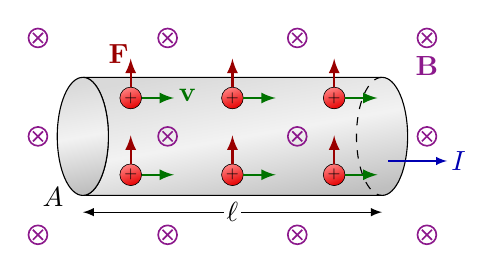
\begin{tikzpicture}
  \def\xmax{3.8}
  \def\ymax{1.25}
  \def\R{0.2}
  \def\Rx{0.26*\ymax}
  \def\Ry{0.6*\ymax}
  \def\L{\xmax}
  \def\NBy{3}
  \def\NBx{4}
  \coordinate (LT) at (0,\Ry);
  \coordinate (LB) at (0,-\Ry);
  \coordinate (RT) at (\L,\Ry);
  \coordinate (RB) at (\L,-\Ry);
  \coordinate (Q) at (0.15*\xmax,0.15*\ymax);
  \def\charge#1#2{
    \node[charge+,draw=black,circle,fill,inner sep=1,scale=0.6] (q) at (#1*\xmax,#2*\Ry) {$+$};
    \draw[vector] (q) --++ (0:0.55);
    \draw[force] (q) --++ (90:0.5);
  }
  
  % CURRENT
  \draw[metal]
    (LB) arc (-90:90:{\Rx} and {\Ry}) --
    (RT) arc (90:-90:{\Rx} and {\Ry}) -- cycle;
  \draw[metal] (0,0) ellipse ({\Rx} and {\Ry});
  \draw[dashed] (RT) arc (90:270:{\Rx} and {\Ry});
  %\draw[metal] (RT) arc (-90:90:{\Rx} and {\Ry});
  
  % CHARGE
  \charge{0.16}{0.65}
  \charge{0.50}{0.65}
  \charge{0.84}{0.65}
  \charge{0.16}{-.65}
  \charge{0.50}{-.65}
  \charge{0.84}{-.65}
  
  % B FIELD
  \foreach \i [evaluate={\y=(\i-\NBy/2-0.5)*2*\ymax/(\NBy-1);}] in {1,...,\NBy}{
    \foreach \j [evaluate={\x=-0.15*\xmax+(\j-1)*1.3*\xmax/(\NBx-1);}] in {1,...,\NBx}{
      \pic at (\x,\y) {Bin};
    }
  }
  \node[Bcol] at (1.15*\xmax,0.71*\ymax) {$\vb{B}$};
  \node at (-0.1*\xmax,-1.02*\Ry) {$A$};
  \node[BFcol] at (0.12*\xmax,1.4*\Ry) {$\vb{F}$};
  \node[veccol] at (0.35*\xmax,0.70*\Ry) {$\vb{v}$};
  \draw[<->] (LB)++(-90:0.17*\ymax) --++ (\L,0) node[midway,fill=white,inner sep=1] {$\ell$};
  \draw[current] (1.02*\xmax,-0.25*\ymax) --++ (0.6*\ymax,0) node[right=-2] {$I$};
  
\end{tikzpicture}


% B FIELD with half circle 3D
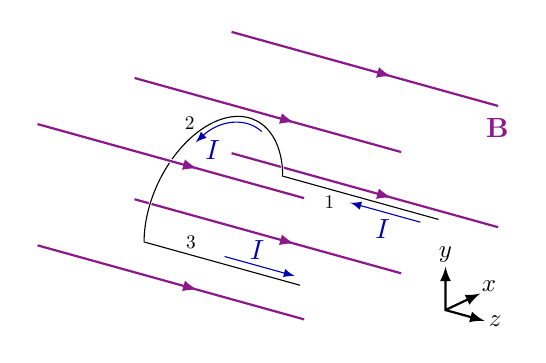
\begin{tikzpicture}[y={(0,1)},z={(0.9,-0.25)},x={(0.8,0.38)}]
  \def\R{1.1}
  \def\a{0.75*\R}
  \def\L{2.2}
  \def\NBx{3}
  \def\NBy{2}
  \coordinate (O) at (-0.7*\R,0,1.8*\L);
  
  % AXES
  \draw[->,thick] (O) --++ (0.5*\R,0,0) node[scale=0.9,above right=-3] {$x$};
  %\draw[->,thick] (O) --++ (0,0.5*\R,0) node[scale=0.9,above=-2] {$y$};
  \draw[<->,thick] (O)++(0,0.5*\R,0) node[scale=0.9,above=-2] {$y$} --
                   (O) --++ (0,0,0.5*\R) node[scale=0.9,right=-2] {$z$};
  %\draw[dashed,very thin] (0,0) coordinate (O) -- (40:\R) coordinate (F);
  
  % CIRCUIT
  \draw
    (\R,0,\L) -- (\R,0,0) arc (0:180:\R) -- (-\R,0,\L);
  \node[below=0,scale=0.7] at (\R,0,0.3*\L) {$1$};
  \node[above=1,scale=0.7] at (110:\R) {$2$};
  \node[above=0,scale=0.7] at (-\R,0,0.3*\L) {$3$};
  
  % B FIELD
  \foreach \i [evaluate={\y=-0.2*\R+(\i-1)*(1.4*\R)/(\NBy-1);}] in {1,...,\NBy}{
    \foreach \j [evaluate={\x=-1.3*\R+(\j-1)*(2.8*\R)/(\NBx-1);}] in {1,...,\NBx}{
      \draw[white,line width=1.5] (\x,\y,-0.6*\L) -- (\x,\y,1.16*\L);
      \draw[BFieldLine=0.6] (\x,\y,-0.55*\L) -- (\x,\y,1.16*\L);
    }
  }
  \draw[white,line width=1] (\R,0,0) arc (0:90:\R) (-\R,0,0) arc (180:140:\R);
  \draw                     (\R,0,0) arc (0:90:\R) (-\R,0,0) arc (180:140:\R);
  \node[Bcol] at (1.4*\R,\R,1.2*\L) {$\vb{B}$};
  
  % CURRENT
  \draw[current] (42:0.94*\R) arc (42:110:0.88*\R) node[right=4,below right=-4] {$I$};
  \draw[current] ( 0.85*\R,0,0.95*\L) --++ (0,0,-0.45*\L) node[midway,left=1,below=-1] {$I$};
  \draw[current] (-0.85*\R,0,0.45*\L) --++ (0,0,0.45*\L) node[midway,left=1,above=-1] {$I$};
  
\end{tikzpicture}


% B FIELD with half circle 2D
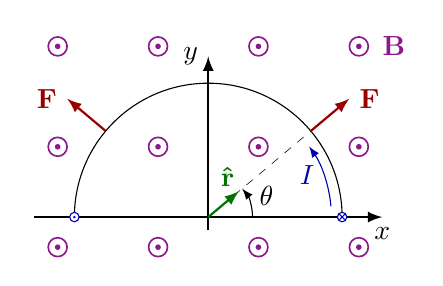
\begin{tikzpicture}
  \def\R{1.7}
  \def\a{0.75*\R}
  \def\NBx{4}
  \def\NBy{3}
  
  % AXES
  \draw[->,thick] (-1.3*\R,0) -- (1.3*\R,0) node[below] {$x$};
  \draw[->,thick] (0,-0.1*\R,0) -- (0,1.2*\R) node[left] {$y$};
  \draw[dashed,very thin] (0,0) coordinate (O) -- (40:\R) coordinate (F);
  \draw[vector] (O) -- (40:0.3*\R) node[above left=-2] {$\vu{r}$};
  
  % B FIELD
  \foreach \i [evaluate={\y=-0.3*\a+(\i-1)*\a;}] in {1,...,\NBy}{
    \foreach \j [evaluate={\x=(\j-\NBx/2-0.5)*\a;}] in {1,...,\NBx}{
      \pic at (\x,\y) {Bout};
    }
  }
  \node[Bcol] at (1.85*\a,1.7*\a) {$\vb{B}$};
  
  % CIRCUIT
  \draw (\R,0) coordinate (R) arc (0:180:\R);
  \draw[current] (5:0.92*\R) arc (5:35:0.92*\R) node[midway,left] {$I$};
  \pic[scale=0.5] at (\R,0) {Bin={Icol,fill=white,line width=0.4}};
  \pic[scale=0.5] at (-\R,0) {Bout={Icol,line width=0.4}};
  \draw pic[->,"$\theta$",draw=black,angle radius=16,angle eccentricity=1.4]
    {angle = R--O--F};
  
  % FORCE
  \draw[force] (F) --++ ( 40:0.5*\a) node[force,right] {$\vb{F}$};
  \draw[force] (140:\R) --++ (140:0.5*\a) node[force,left] {$\vb{F}$};
  
\end{tikzpicture}


% B FIELD perpendicular to square circuit 3D
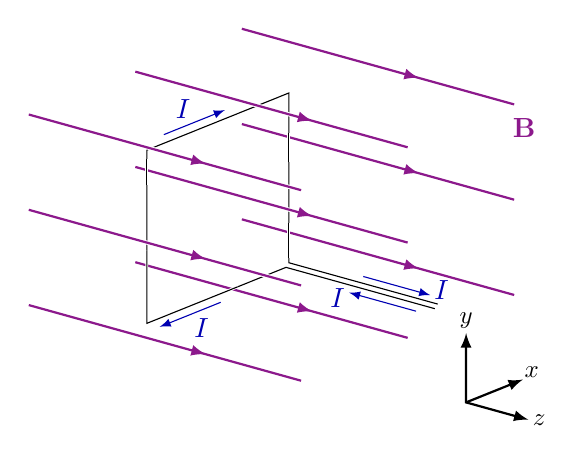
\begin{tikzpicture}[y={(0,1)},z={(0.9,-0.25)},x={(0.82,0.33)}]
  \def\W{2.2}
  \def\L{2.1}
  \def\a{0.75*\R}
  \def\NBx{3}
  \def\NBy{3}
  \coordinate (O) at (0.1*\W,0,2.05*\L);
  
  % AXES
  \draw[->,thick] (O) --++ (0.4*\W,0,0) node[scale=0.9,above right=-3] {$x$};
  \draw[<->,thick] (O)++(0,0.4*\W,0) node[scale=0.9,above=-2] {$y$} --
                   (O) --++ (0,0,0.4*\W) node[scale=0.9,right=-2] {$z$};
  
  % CIRCUIT
  \draw
    (\W,0.02*\W,\L) -- (\W,0.02*\W,0) -- (\W,\W,0) -- (0,\W,0) -- (0,0,0) -- (0.98*\W,0,0) -- (0.98*\W,0,\L);
  %\node[above=1,scale=0.7] at (\W,0,0.4*\L) {$1$};
  %\node[below=1,scale=0.7] at (\W,0,0.4*\L) {$6$};
  %\node[right=1,scale=0.7] at (\W,\W/2) {$2$};
  %\node[above=1,scale=0.7] at (0.3*\W,\W) {$3$};
  %\node[left=1, scale=0.7] at (0,0.6*\W) {$4$};
  %\node[below=1,scale=0.7] at (0.4*\W,0) {$5$};
  
  % B FIELD
  \foreach \i [evaluate={\y=(\i-1)*(1.1*\W)/(\NBy-1);}] in {1,...,\NBy}{
    \foreach \j [evaluate={\x=-0.15*\W+(\j-1)*(1.5*\W)/(\NBx-1);}] in {1,...,\NBx}{
      \draw[white,line width=1.5] (\x,\y,-0.6*\L) -- (\x,\y,1.16*\L);
      \draw[BFieldLine=0.65] (\x,\y,-0.65*\L) -- (\x,\y,1.18*\L);
    }
  }
  \draw[white,line width=1] (0,0.42*\W,0) -- (0,0,0) -- (0.64*\W,0,0);
  \draw                     (0,0.42*\W,0) -- (0,0,0) -- (0.64*\W,0,0);
  \draw[white,line width=1] (0,0.80*\W,0) -- (0,0.95*\W,0);
  \draw                     (0,0.80*\W,0) -- (0,0.95*\W,0);
  \draw[white,line width=1] (\W,0.05*\W,0) -- (\W,0.25*\W,0);
  \draw                     (\W,0.05*\W,0) -- (\W,0.25*\W,0);
  \draw[white,line width=1] (\W,0.60*\W,0) -- (\W,0.77*\W,0);
  \draw                     (\W,0.60*\W,0) -- (\W,0.77*\W,0);
  \node[Bcol] at (1.4*\W,0.95*\W,1.2*\L) {$\vb{B}$};
  
  % CURRENT
  \draw[current] (\W,0.06*\W,0.50*\L) --++ (0,0,0.45*\L) node[above=2,right=-2] {$I$};
  \draw[current] (0.90*\W,0,0.95*\L) --++ (0,0,-0.45*\L) node[below=2,left=-2] {$I$};
  \draw[current] (0.12*\W,1.05*\W,0) --++ (0.45*\L,0,0) node[midway,above left=-2] {$I$};
  \draw[current] (0.52*\W,-0.05*\W,0) --++ (-0.45*\L,0,0) node[midway,below right=-2] {$I$};
  
\end{tikzpicture}


% B FIELD perpendicular to square circuit 2D
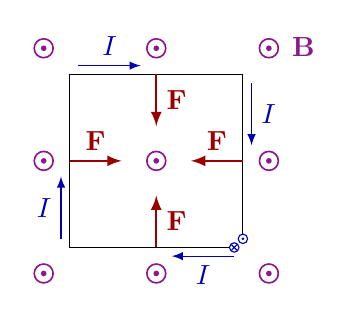
\begin{tikzpicture}
  \def\H{2.2}
  \def\W{2.2}
  \def\NB{3}
  
  % ELECTRIC FIELD
  \foreach \i [evaluate={\y=-0.15*\W+(\i-1)*1.3*\H/(\NB-1);}] in {1,...,\NB}{
    \foreach \j [evaluate={\x=-0.15*\W+(\j-1)*1.3*\W/(\NB-1);}] in {1,...,\NB}{
      \pic at (\x,\y) {Bout};
    }
  }
  \node[Bcol] at (1.35*\W,1.16*\W) {$\vb{B}$};
  
  % CIRCUIT
  \draw (0,0) rectangle (\W,\H);
  \draw[current] ( 0.05*\W, 1.05*\H) --++ ( 0.36*\W,0) node[midway,above] {$I$};
  \draw[current] ( 0.95*\W,-0.05*\H) --++ (-0.36*\W,0) node[midway,below] {$I$};
  \draw[current] ( 1.05*\W, 0.95*\H) --++ (0,-0.36*\H) node[midway,right] {$I$};
  \draw[current] (-0.05*\W, 0.05*\H) --++ (0, 0.36*\H) node[midway,left] {$I$};
  \fill[white] (\W,0) circle (0.06);
  %\fill (\W,0.03*\W) circle (0.04);
  %\fill (0.97*\W,0) circle (0.04);
  \pic[scale=0.5] at (0.95*\W,0) {Bin={Icol,fill=white,line width=0.4}};
  \pic[scale=0.5] at (\W,0.05*\H) {Bout={Icol,line width=0.4}};
  
  % FORCE
  \draw[force] (\W/2,\H) --++ (0,-0.3*\H) node[force,midway,right] {$\vb{F}$};
  \draw[force] (\W/2, 0) --++ (0, 0.3*\H) node[force,midway,right] {$\vb{F}$};
  \draw[force] (\W,\H/2) --++ (-0.3*\W,0) node[force,midway,above] {$\vb{F}$};
  \draw[force] ( 0,\H/2) --++ ( 0.3*\W,0) node[force,midway,above] {$\vb{F}$};
  
\end{tikzpicture}


% B FIELD along circuit
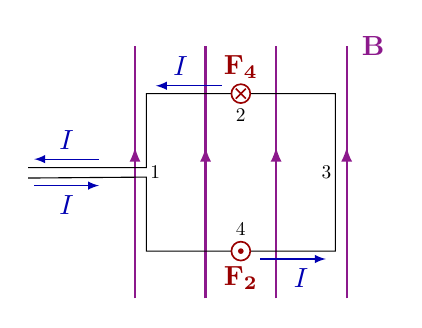
\begin{tikzpicture}
  \def\a{0.03}
  \def\L{1.5}
  \def\W{2.4}
  \def\H{2.0}
  \def\NB{4}
  
  % MAGNETIC FIELD
  %\foreach \i [evaluate={\y=(\i-0.5)*0.8*\H/(\NB-0.5);}] in {1,...,\NB}{
  %  \draw[BFieldLine] (-0.3*\W,\y) -- (1.2*\W,\y);
  %  \draw[BFieldLine] (-0.3*\W,-\y) -- (1.2*\W,-\y);
  %}
  \foreach \i [evaluate={\x=-0.06*\W+(\i-1)*1.12*\W/(\NB-1);}] in {1,...,\NB}{
    \draw[BFieldLine=0.6] (\x,-0.8*\H) -- (\x,0.8*\H);
  }
  \node[Bcol] at (1.2*\W,0.8*\H) {$\vb{B}$};
  
  % CIRCUIT
  \draw (-\L,\a*\H) -| (0,\H/2) -| (\W,-\H/2) -| (0,-\a*\H) -- (-\L,-\a*\W);
  \draw[current,<-] (-0.95*\L, 2.8*\a*\H) --++ (0.55*\L,0) node[midway,above] {$I$};
  \draw[current] (-0.95*\L,-2.8*\a*\H) --++ (0.55*\L,0) node[midway,below] {$I$};
  \draw[current,<-] ( 0.05*\W, 0.55*\H) --++ (0.35*\W,0) node[midway,left=3,above] {$I$};
  \draw[current,<-] ( 0.95*\W,-0.55*\H) --++ (-0.35*\W,0) node[midway,right=3,below] {$I$};
  \pic at (\W/2, \H/2) {Bin={BFcol,fill=white}};
  \pic at (\W/2,-\H/2) {Bout={BFcol}};
  \node[BFcol,above=2] at (\W/2, \H/2) {$\vb{F_4}$};
  \node[BFcol,below=2] at (\W/2,-\H/2) {$\vb{F_2}$};
  \node[right=-1,scale=0.7] at (0,0) {$1$};
  \node[left=-1,scale=0.7] at (\W,0) {$3$};
  \node[above=3,scale=0.7] at (\W/2,-0.5*\H) {$4$};
  \node[below=3,scale=0.7] at (\W/2, 0.5*\H) {$2$};
  
\end{tikzpicture}


\end{document}
